\begin{questions}
	
\question
\exonly{		
	Calcola senza aiutarti con la calcolatrice:
\begin{multicols}{3}
	\begin{parts}
		\part $ \dfrac{2}{3} + \dfrac{3}{4} = $
		\part $ \dfrac{7}{6} - \dfrac{5}{8} + \dfrac{4}{9} = $
		\part $ \dfrac{1}{15} - \dfrac{2}{5} + \dfrac{3}{25} = $
		\part $ \dfrac{2}{6} + \dfrac{5}{15} - \dfrac{12}{18} = $
		\part $ \dfrac{a}{3} + \dfrac{2}{5} - \dfrac{4}{3} = $
		\part $ \dfrac{1}{x} + \dfrac{3}{5} - \dfrac{3}{2x} = $
		\part $ \dfrac{\dfrac{1}{3} + \dfrac{1}{5}}{\dfrac{4}{15}-\dfrac{2}{6}} = $
		\part $ \dfrac{\dfrac{2}{3} \cdot (\dfrac{1}{6} + \dfrac{1}{2})}{\dfrac{3}{4}-\dfrac{3}{10}} = $
		\part $ \dfrac{2}{3} \cdot \dfrac{1}{5} + \dfrac{\dfrac{3}{2}}{\dfrac{7}{5}} = $
		\part $ \dfrac{4}{9} \cdot \dfrac{6}{10} + \dfrac{\dfrac{8}{30}}{\dfrac{6}{5}} = $
	\end{parts}	
\end{multicols} }
\solonly{Calcolatrice CAS}

\question
\exonly{
		Calcola senza aiutarti con la calcolatrice:
\begin{multicols}{2}
	\begin{parts}
		\part $ 2^3 \cdot 2^{-2} \cdot 2^4 \cdot 2^{-1} =$
		\part $ \dfrac{3^2\cdot 3^3}{3^4} = $
		\part $ \dfrac{5^3\cdot 5^{-2}}{5^4 \cdot 5^{-3}} = $
		\part $ \left(2^2\right)^2 \cdot \left(2^{-1}\right)^3 \cdot \left(2^2\right)^{-2} $
		\part $ \left(3^2\right)^{-1} \cdot \left(2^{-2}\right)^{-1} \cdot \left(6^2\right)^2 =$
		\part $ \left[\left(\dfrac{1}{5}\right)^{2}\cdot\left(\dfrac{1}{5}\right)^{3}\right]^{2}\cdot\left(\dfrac{1}{5}\right)^{-7} = $
		\part $ \dfrac{3^5 \cdot 2^4}{6^3} = $
		\part $ \dfrac{\left[\left(\dfrac{3}{4}\right)^{-1}\right]^{2} \cdot \left(\dfrac{2}{9}\right)^{-2}}{\left(\dfrac{1}{6}\right)^{-3}} = $
		\part $ \left\lbrace \dfrac{\left[\left(3^{2}\right)^{-1}\right]^{2}}{\left(\dfrac{1}{3}\right)^{-3}}\right\rbrace ^{-1} \cdot \left[\left(\dfrac{2}{5}\right)^{2} \cdot \left(\frac{5}{6}\right)^{2}\right]   = $
	\end{parts}
\end{multicols}
 }
	

\question
\exonly{Semplifica e calcola senza utilizzare la calcolatrice: }

%\exonly{
%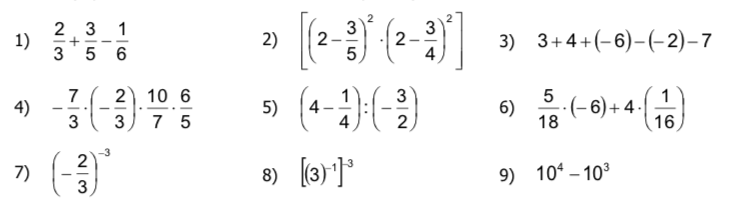
\includegraphics[scale=0.6]{test-form-1}
%
%}
\begin{minipage}{\linewidth}
	\begin{multicols}{2}
\begin{parts}
	\part
	\exonly{$\dfrac{3}{3}+\dfrac{3}{5}-\dfrac{1}{6}$ }
	\solonly{$\dfrac{11}{10}$ }
	
	\part
	\exonly{ $\left[ \left( 2-\dfrac{3}{5}\right) ^2 \cdot \left( 2-\dfrac{3}{4}\right) ^2 \right] $  }
	\solonly{$\dfrac{49}{16}$ }
	
	\part
	\exonly{$3+4+(-6)-(-2)-7$ }
	\solonly{$-4$ }
	
	\part
	\exonly{$-\dfrac{7}{3} \cdot \left( -\dfrac{2}{3}\right) \cdot \dfrac{10}{7} \cdot \dfrac{6}{5} $ }
	\solonly{$\dfrac{8}{3}$ }
	
	\part
	\exonly{$\left( 4-\dfrac{1}{4}\right) \div \left( -\dfrac{3}{2}\right) $ }
	\solonly{$-\dfrac{5}{2}$ }
	
	\part
	\exonly{$\dfrac{15}{18}\cdot\left( -6 \right) +4\cdot \left( \dfrac{1}{16}\right) $ }
	\solonly{$-\dfrac{17}{12}$ }
	
	\part
	\exonly{$\left( -\dfrac{2}{3}\right) ^{-3}$ }
	\solonly{$-\dfrac{27}{8}$ }
	
	\part
	\exonly{$\left[ \left( 3\right) ^{-1}\right] ^{-3}$ }
	\solonly{$27$ }
	
	\part
	\exonly{$10^4-10^3$ }
	\solonly{$9000$ }
\end{parts}
\end{multicols}
\end{minipage}

%\solonly{
%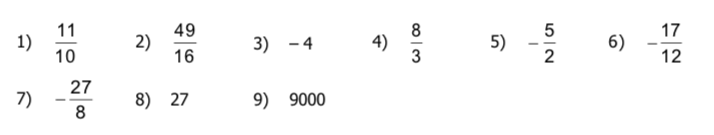
\includegraphics[scale=0.6]{test-form-1-sol}
%}

%\exnewpage
\question
\exonly{
	Calcola senza aiutarti con la calcolatrice:
\begin{multicols}{2}
	\begin{parts}
		\part $ x - 2x + 3x - 4x + 5x - 6x =$
		\part $ a^2 + 2a -3a^2 +a = $
		\part $ a^2 \cdot a^3 = $
		\part $ \left(a^2\right)^2 + a\cdot a^3 - \left(a^6\right)^{-2} =$
		\part $ x^{-2} \cdot \left(x^2\right)^3 = $
		\part $ \dfrac{9 \cdot a^2 \cdot b^3 }{3 \cdot a^{-2} \cdot b^5} = $
		\part $ \dfrac{2 \cdot a^3 \cdot b^2 }{3 \cdot a \cdot b^4} \cdot \dfrac{a+b}{a}  = $
		\part $ a\left(a(a^{-1}+1) + a(a-1)\right) =$
\end{parts}
\end{multicols}
 }



\end{questions}